\documentclass{article}
\usepackage[utf8]{inputenc}
\usepackage{dirtytalk}
\usepackage{bussproofs}
\usepackage{comment}
\usepackage{mathtools}
\usepackage{amsmath}
\usepackage{amsfonts}
\usepackage{amssymb}
\usepackage{indentfirst}
\DeclarePairedDelimiter\ceil{\lceil}{\rceil}
\DeclarePairedDelimiter\floor{\lfloor}{\rfloor}
\usepackage{pgfplots}
\usepackage{graphicx}
\usepackage{pgf}
\usepackage{pgfpages}



\begin{document}
\par The Jacobi theta function is a interesting special function, whose properties we will need in the derivation of the Riemann functional equation for the zeta function. I plan to make a post on it soon so I need to lay out the groundwork here with this functional equation. The theta function is interesting, because it's Mellin Transform is the zeta function itself. Let's begin with a definition.
\begin{equation*}
    \vartheta(x)=\sum_{n=-\infty}^{\infty} e^{-\pi n^2x}
\end{equation*}
To prove it's functional equation, we will utilize the Poisson Summation Formula. It states
\begin{equation*}
    \sum_{n=-\infty}^{\infty} f(n)= \sum_{k=-\infty}^{\infty} \underbrace{\int_{-\infty}^{\infty} f(y)e^{-2\pi i k y}\,y}_{=\hat{f}(k), \text{Fourier transform}}
\end{equation*}
The proof of this result is not motivated by our current intentions, and is not necessary for our goals so it will be omitted. Now, let's apply this transform to our function. 
\begin{equation*}
    \begin{split}
        \sum_{n=-\infty}^{\infty} e^{-\pi n^2x}&= \sum_{k=-\infty}^{\infty} \int_{-\infty}^{\infty}e^{-\pi y^2x}e^{-2\pi i k y}\,dy \\
         \vartheta(x)&= \sum_{k=-\infty}^{\infty} \int_{-\infty}^{\infty} e^{-\pi y^2x-2\pi i k y}\,dy \\
         &= \sum_{k=-\infty}^{\infty} \int_{-\infty}^{\infty} e^{{-\pi x( y^2+2 \frac{iyk}{x})}}\,dy 
    \end{split} 
\end{equation*} Now we can `complete the square' inside the exponential by adding and subtracting a term. 
\begin{equation*}
\begin{split}
     y^2+2 i y\frac{k}{x}&= y^2+2 i y\frac{k}{x}+\frac{i^2k^2}{x^2}-\frac{i^2k^2}{x^2} \\
     &= \left(y+\frac{ik}{x}\right)^2+\frac{k^2}{x^2}
     \end{split}
\end{equation*}
So,
\begin{equation*}
    \begin{split}
        \vartheta(x)&= \sum_{k=-\infty}^{\infty} \int_{-\infty}^{\infty} e^{-\pi x\left(\left(y+\frac{ik}{x}\right)^2+\frac{k^2}{x^2}\right)} \,dy \\ 
        &= \sum_{k=-\infty}^{\infty} e^{-\pi k^2 \frac{1}{x}}\int_{-\infty}^{\infty} e^{-\pi x\left(y+\frac{ik}{x}\right)^2}\,dy
    \end{split}
\end{equation*}
We will now perform a substitution $z=y+i\frac{k}{x}$, $dy=dz$, which will shift our bounds accordingly. This will transform our real integral into a path integral in the complex plane. 
\begin{equation*}
    \vartheta(x)=\sum_{k=-\infty}^{\infty} e^{-\pi k^2 \frac{1}{x}}\underbrace{\int_{-\infty+i\frac{k}{x}}^{\infty+i\frac{k}{x}} e^{-\pi xz^2}\,dz}_{=I}  \, 
\end{equation*}
We notice that the function inside the integrand is everywhere holomorphic, in other words it has no poles or discontinuities. That means if we can integrate it on any closed contour, this integral will be 0. Let's consider a rectangle with height $i\frac{k}{x}$ and length of $R$, and we will then take the limit as $R$ goes to infinity.
\begin{figure}[htp]
    \centering
    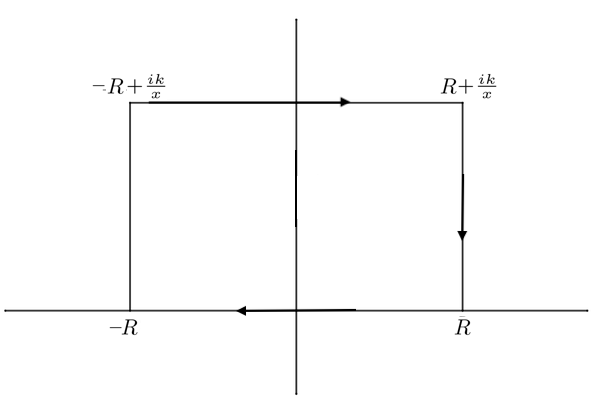
\includegraphics[width=12cm]{contour.png}
    \caption{Graph of Contour C in the Complex Plane}
    \label{fig:Desmos}
\end{figure} 
Now we break up the contour integral into parts. Letting $f(z)=$ the integrand,
\begin{equation*}
    \oint_{C} f(z)\,dz=\int_{+R}^{-R} f(z)\,dz+\int_{-R}^{-R+i\frac{k}{x}} f(z)\,dz+\int_{-R+i\frac{k}{x}}^{+R+i\frac{k}{x}} f(z)\,dz+\int_{+R+i\frac{k}{x}}^{+R} f(z)\,dz
\end{equation*}
As discussed earlier, we also have 
\begin{equation*}
     \oint_{C} f(z)\,dz=0,
\end{equation*} 
So we can write 
\begin{equation*}
    \int_{-R+i\frac{k}{x}}^{+R+i\frac{k}{x}} f(z)\,dz=\int_{-R}^{+R} f(z)\,dz-\underbrace{\int_{+R+i\frac{k}{x}}^{+R} f(z)\,dz}_{I_1}-\underbrace{\int_{-R}^{-R+i\frac{k}{x}} f(z)\,dz}_{I_2}
\end{equation*}
Both of these integrals $I_1$ and $I_2$ will approach 0 as $R \rightarrow \infty$, which we can show using the ML inequality:
\begin{equation*}
    \left|\int_{C} f(z)\,dz\right| \leq ML
\end{equation*}
where M is the maximum value of $f$ on $C$, and $L$ is the length of the curve $C$. To see a proof an explanation, see my most recent complex analysis series post. \par Now, we know that the length, $L$, of both curves is finite (More specifically, both have a length of $k/x$). However, if we take the limit as R approaches infinity of our function f, the real part of any complex number $z$ on this curves will approach $\pm \infty$. Since,
\begin{equation*}
    \lim_{z\rightarrow \pm \infty}  e^{-\pi xz^2} = 0,
\end{equation*}
then we have
\begin{equation*}
    \begin{split}
        I_1,I_2 &\leq 0\cdot \frac{k}{x}\\
        &= 0
    \end{split}
\end{equation*}
Thus, both of these integrals will evaluate to 0. Putting it all together, 
\begin{equation*}
     \int_{-\infty+i\frac{k}{x}}^{+\infty+i\frac{k}{x}} e^{-\pi xz^2}\,dz=\int_{-\infty}^{+\infty} e^{-\pi xz^2}\,dz
\end{equation*} 
This is now a much easier integral to evaluate. We look at the integral cleverly such that
\begin{equation*}
    \int_{-\infty}^{+\infty} e^{-\pi xz^2}\,dz=\int_{-\infty}^{+\infty} e^{-(\sqrt{\pi x}z)^2}\,dz
\end{equation*}
Now letting $u=\sqrt{\pi x}z$, we have
\begin{equation*}
     \int_{-\infty}^{+\infty} e^{-\pi xz^2}\,dz=\frac{1}{\sqrt{\pi x}}\int_{-\infty}^{+\infty} e^{-u^2}\,du
\end{equation*}
And once we substitute in the value for the standard Gaussian integral, 
\begin{equation*}
\begin{split}
    \int_{-\infty}^{+\infty} e^{-\pi xz^2}\,dz&=\frac{1}{\sqrt{\pi}\sqrt{x}}\sqrt{\pi} \\
    &= \frac{1}{\sqrt{x}}
    \end{split}
\end{equation*}
Now let us recall from earlier,
\begin{equation*}
    \vartheta(x)=\sum_{k=-\infty}^{\infty} e^{-\pi k^2 \frac{1}{x}}\underbrace{\int_{-\infty+i\frac{k}{x}}^{\infty+i\frac{k}{x}} e^{-\pi xz^2}\,dz}_{=I}  \, 
\end{equation*} 
If we replace the value we found for this integral, 
\begin{equation*}
    \vartheta(x)=\frac{1}{\sqrt{x}}\sum_{k=-\infty}^{\infty} e^{-\pi k^2 \frac{1}{x}}
\end{equation*}
However, the sum on the RHS is simply the definition of the theta function with input $1/x$. So,
\begin{equation*}
     \vartheta(x)=\frac{1}{\sqrt{x}}\vartheta\left(\frac{1}{x}\right)
\end{equation*}
Hence, proven. We will use this result in the Riemann functional equation derivation. 
\end{document}
